\chapter{绪论}\label{chapter_introduction}
\graphicspath{{chapter1/figure/}}
%\bibliographystyle{unsrt}

\section{研究背景}

本论文的研究主要基于两大背景:\uline{Moore定律的最终终结}以及\uline{脑科学,人工智能研究的兴起}。

Moore定律是由Intel的创始人Gordon Moore于1965年提出的一个经验规律,其描述的内容是:在价格不变的情况下,集成电路上可容纳的元件的数目,约每隔18-24个月便会增加一倍,性能也因此提升一倍。\cite{wikipedia_moores_law}

\begin{figure}[htbp]
   \centering
   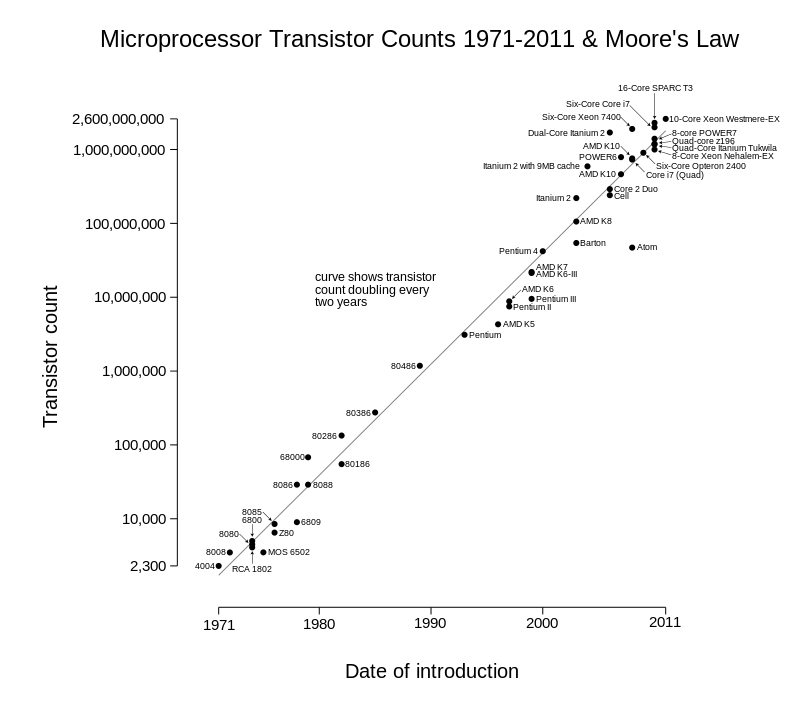
\includegraphics[width=0.5\textwidth]{MooreLaw.png} % requires the graphicx package
   \caption{Moore定律:CPU中随着时间指数级增长的晶体管规模}
   \label{fig:moore}
\end{figure}

Moore定律是近50年来信息技术得以迅速发展的重要保障,如图\ref{fig:moore},伴随着晶体管规模的增长,由CPU体现的计算机运算能力也实现了指数级增长,由此促使了人类生活发生了巨大变化。

然而,随着微纳加工逐渐逼近极限,传统的硅基集成电路已经做到尺寸小于10nm的时候,由于加工成本的提升,热效应逐渐明显和量子隧穿效应的出现,传统半导体工艺发展集成电路已经走到了尽头。Gordon Moore于2015年已经公开宣称:“Moore定律十年以内将要结束。”\cite{moore2015declare}

与此同时,人们对于计算的需求却在日益增加。于是,人们从算法、电路、硬件各个层面上探讨如何高效地提升计算能力。一种常见的方法是,改变以前的计算机组织架构,引入一些专用的计算单元来加速某些特定需求的计算。一个常见的专用计算模块便是GPU(Graphics Processing Unit),其通过大量的并行计算结构和有效的内存分配,可以有效地处理图形渲染,矩阵运算等任务。\cite{wikipedia_gpu}

常见的计算任务除了大量的矩阵运算、图形渲染以外,还有一种日益增长的需要,就是进行模式识别与机器学习,譬如人脸识别、指纹识别、数据预测等等。于是,一种专门适用于进行模式识别、机器学习的电路模块可以很好地平衡通用性与计算效率的需要,有很大的市场需求。

另一方面,随着神经科学、认知心理学和计算机科学的不断进步,人工智能领域的发展十分迅速。

从生物学上来讲,由于研究方法、实验手段日益成熟(荧光成像、核磁共振成像、脑电波),人们对于大脑的神经结构有着日益完善的了解,由此展开的类脑结构计算,脑机接口的研究不断深入;IBM的TrueNorth研究团队\cite{brainchip2014}对于电路搭建实现类脑结构已经做出了喜人的结果。(图\ref{fig:truenorth})
从计算机科学上来讲,在神经科学的启发下,通过结合统计学、统计物理的研究成果,一门新兴的学科——机器学习产生了广泛的应用。

\begin{figure}[htbp]
   \centering
   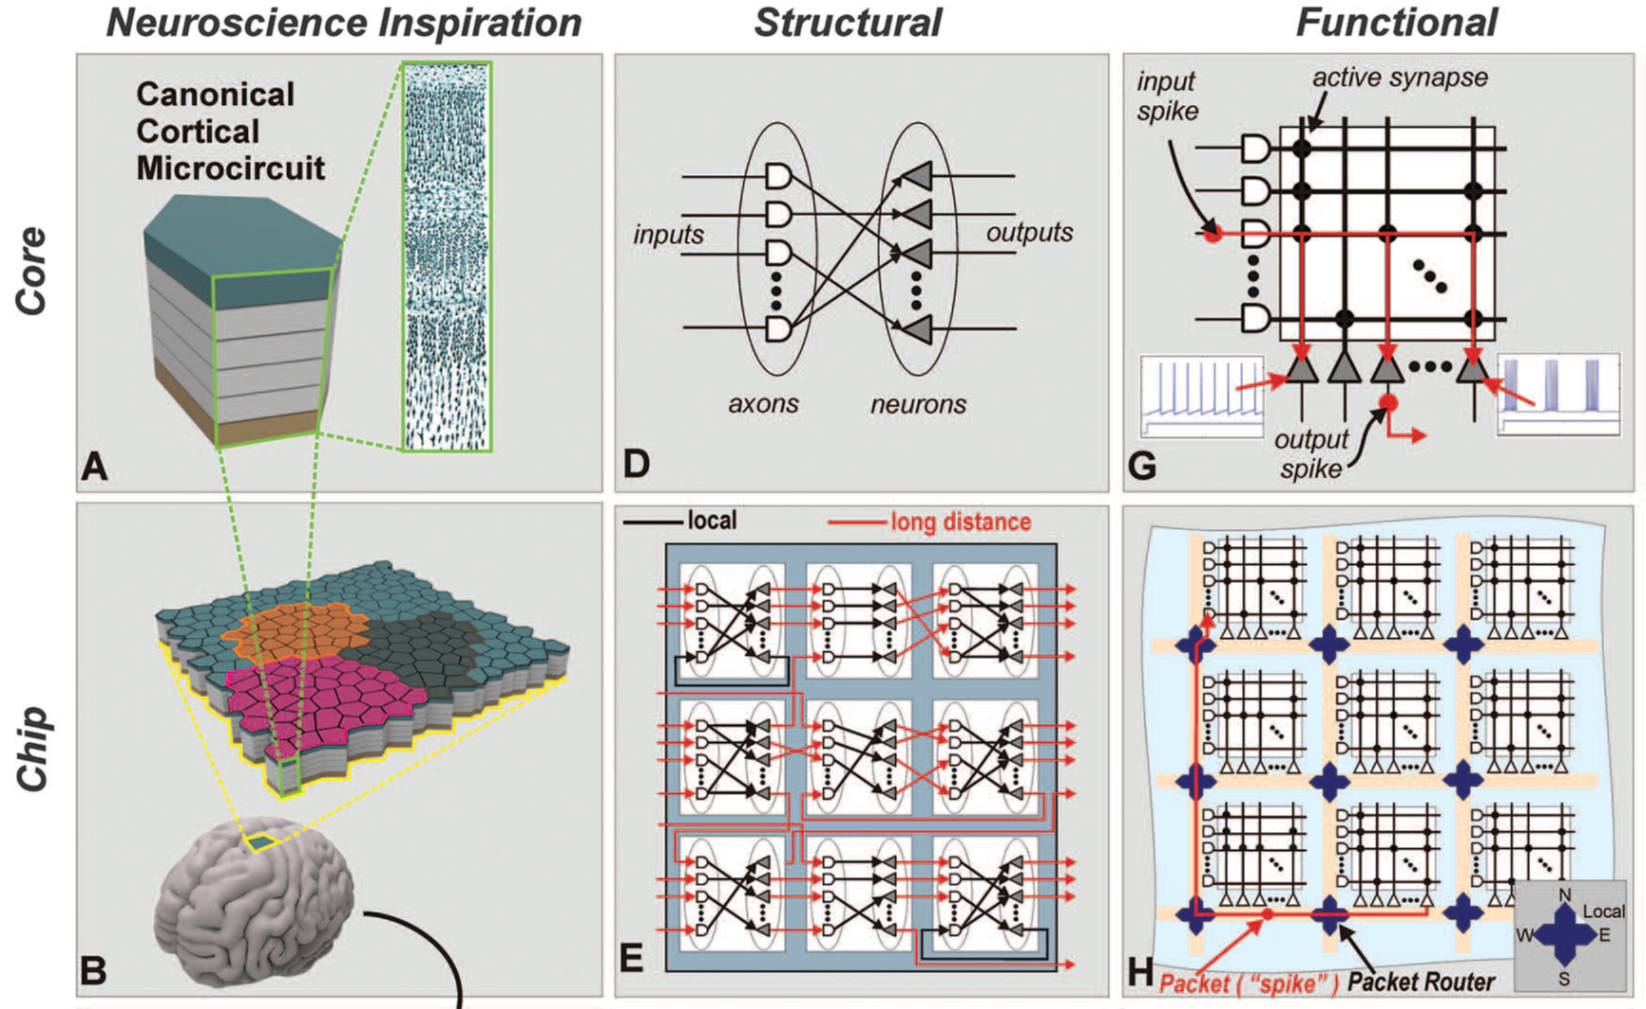
\includegraphics[width=0.7\textwidth]{TrueNorth.png} % requires the graphicx package
   \caption{TrueNorth类脑结构实现原理}
   \label{fig:truenorth}
\end{figure}

综合以上两个方面,人们想通过专用电路的设计实现特定的模式识别功能;并以此为基础,搭建类脑的神经网络,研究类脑结构的计算框架。

\section{研究目的与意义}
\subsection{现有解决方法}
在专用电路进行机器学习领域,中科院计算技术研究所的陈天石,陈云霁等人推出的“寒武纪”处理器系列处于国际领先的地位\cite{Chen2014DianNao},其设计的“DianNaoYu”指令集能够很好的实现卷积神经网络(Convolutional Neural Network)和深度神经网络(Deep Neural Network)的通用架构设计。图\ref{fig:diannao}为其“DianNao”处理器内部的实现加速的硬件架构。

\begin{figure}[htbp]
   \centering
   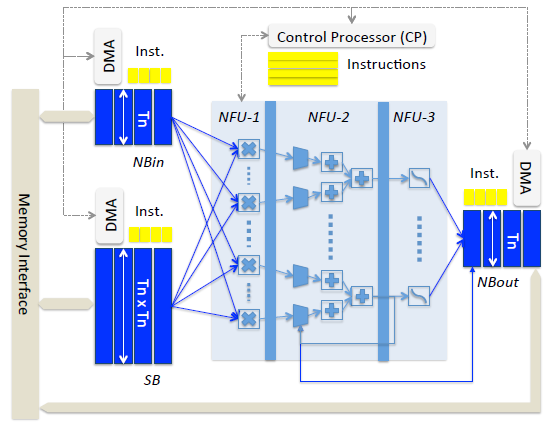
\includegraphics[width=0.6\textwidth]{DianNao.png} % requires the graphicx package
   \caption{"寒武纪"系列电脑采用的硬件模块设计}
   \label{fig:diannao}
\end{figure}

除了利用数字电路进行网络架构设计以外,利用模拟电路搭建“模拟神经元”的方法也得到了相关的研究。图\ref{fig:clustering}\cite{Lu2014An}为一种聚类算法的神经元的模拟电路架构。

\begin{figure}[htbp]
   \centering
   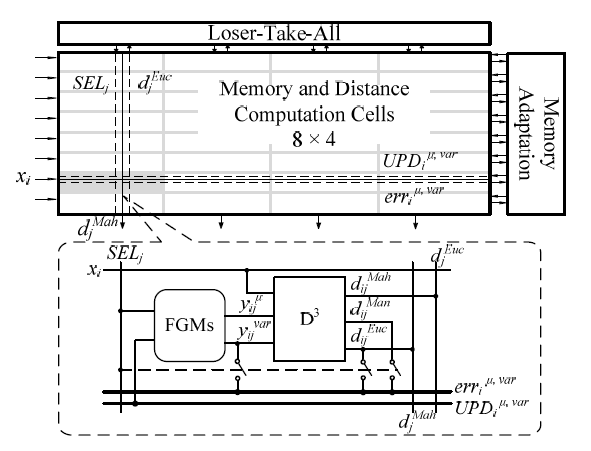
\includegraphics[width=0.6\textwidth]{OnlineClustering.png} % requires the graphicx package
   \caption{Online Clustering算法的模拟神经元架构}
   \label{fig:clustering}
\end{figure}

“寒武纪”系列以及相关的基于卷积神经网络的专用电路方法具有一定的局限性。卷积神经网络应用于静态图像处理取得了巨大成功,但是其在处理时间依赖的问题上面具有严重的局限性。

\subsection{本研究的目的与意义}
本研究试图研究一个对于动态识别具有良好效果的深度学习算法(DeSTIN),先对其算法进行可靠性研究,判断其对于静态、动态图像的识别能力;然后对该算法进行量化,判断其转换为定点数算法之后的可行性;再对该算法进行专用的数字电路设计,并对其进行仿真测试与综合。

在学习算法上,DeSTIN算法相比较于卷积神经网络算法具有本质上的动态识别特性,能够更好更快地进行动态识别处理;与此同时,通过识别扫描的方法,DeSTIN算法能够有效地处理静态图像的识别问题。

与此同时,DeSTIN算法具有并行特性以及参数设置上对于数字电路设计的天然优势。 通过专用数字电路的设计,比较于普通的CPU架构编程实现的算法,我们可以通过减少程序读取、转译,数据传送过程的时间损耗,高效率地使用存储;硬件计算具有天然的并行特性,加上流水线结构实现能够使得整个学习过程较为高效。 

而相对于模拟电路设计实现而言,数字电路设计架构相对简单,具有通用性、可移植性;数字电路可以在前期通过量化的方法进行模拟测试,有成熟的数字电路仿真测试软件,便于综合。

%\bibliography{reference}